\documentclass{beamer}

\usepackage[russian]{babel}
\usepackage[utf8]{inputenc}
\usepackage[outputdir=cache]{minted}

\usetheme{Madrid}
\usecolortheme{dove}
\setbeamertemplate{blocks}[rounded][shadow=false]

\title[]{Приложения комплексных чисел к решению геометрических задач}
\institute[]{ФГБОУ ВО «Вятский государственный университет»}
\date{\today}
\author[ ]{Студент ПМИб-2301-52-00 Ступников Григорий Евгеньевич \and К.ф-м.н Пушкарев Игорь Александрович}

\newcommand\frametitleSpec[1]{%
\frametitle{#1}
\section{#1}%
}


% set captions with numbers
\setbeamertemplate{caption}[numbered]

\begin{document}
\begin{frame}
    \centering\includegraphics[width=0.4\textwidth]{images/vyatsu_logo.png}\\
    \titlepage
\end{frame}
\begin{frame}
    \frametitle{План доклада}

    \tableofcontents

\end{frame}
\begin{frame}
    \frametitleSpec{Введение}
    Метод комплексных чисел -- это расширение аналитического метода (т.е задача решается без необходимости графических построений).
    \begin{enumerate}
        \item Проблема состоит в том, что для данного метода отсутствуют программные материалы для внедрения в среду самостоятельного и школьного обучения.
        \item Целью данной работы является изучение метода комплексных чисел при решении геометрических задач, реализация программной верификации решения выбранных задач. Для достижения цели необходимо выполнить следующие задачи:
              \begin{itemize}
                  \item Изучить имеющиеся способы применения алгебры комплексных чисел при решении геометрических задач.
                  \item Выбрать задачи, на которых будет рассматриваться практическое применение метода.
                  \item Решение задач с применением метода комплексных чисел и без них
                  \item Сравнение решений задач.
                  \item Реализация программной верификации решения задач с применением метода.
              \end{itemize}
    \end{enumerate}

\end{frame}
\begin{frame}
    \frametitleSpec{Основы метода}
    \begin{columns}
        \begin{column}{0.5\textwidth}
            Комплексное число \(z\) -- число вида $x + iy$, где $x,y \in \mathbf{R}, i = \sqrt{-1},z \in \mathbf{C}, \mathbf{C}$ - поле комплексных чисел. У числа \(z\) можно выделить действительную $x = Re(z)$ и мнимую $y=Im(z)$ части.
        \end{column}
        \begin{column}{0.5\textwidth}
            \begin{figure}
                \centering
                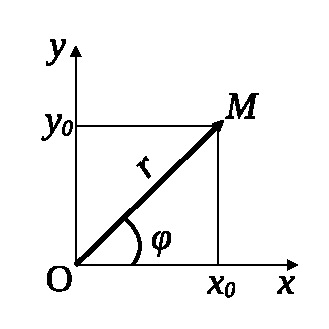
\includegraphics[width=1\textwidth]{images/img1}
                \caption{Изображение числа \(z\) на плоскости}
                \label{img1}
            \end{figure}
        \end{column}
    \end{columns}
\end{frame}
\begin{frame}
    \frametitleSpec{Задачи}
    \subsection{Задача 1}
    \begin{block}{Задача 1}
        Постановка задачи:

        Доказать, что если некоторая прямая пересекает прямые, содержащие стороны \(BC\), \(CA\), \(AB\) треугольника \(ABC\), в точках \(A_1\) , \(B_1\) , \(C_1\) соответственно, то середины отрезков \(AA_1\) , \(BB_1\) , \(CC_1\) коллинеарны.

        \begin{figure}[h]
            \centering
            \includegraphics[width=0.4\textwidth]{images/task1.png}
            \label{task1}
        \end{figure}
    \end{block}
\end{frame}
\begin{frame}

    \begin{block}{Задача 1}
        Решение задачи:
        Кратко
    \end{block}
\end{frame}
\begin{frame}
    \begin{block}{Задача 1}
        \begin{block}{Алгоритм программного решения задачи}
            На вход программы передаются координаты свободных точек, в данном примере это координаты точек \(A,B,C,A_1\). По данным входным данным строится прямая, пересекающая стороны \(BC\), \(CA\), \(AB\) треугольника \(ABC\), в точках \(A_1\) , \(B_1\) , \(C_1\).
        \end{block}
    \end{block}
\end{frame}
\begin{frame}
    (Таблицы с результатами)
\end{frame}
\begin{frame}
    \frametitle{Задачи}

    \subsection{Задача 1}
    \begin{block}{Задача 1}
        \begin{block}{Алгоритм программного решения задачи}
            t
        \end{block}
    \end{block}

\end{frame}
\end{document}
